%!TEX program = xelatex
% 完整编译方法 1 pdflatex -> bibtex -> pdflatex -> pdflatex
% 完整编译方法 2: xelatex -> bibtex -> xelatex -> xelatex
\documentclass[lang=cn,11pt]{elegantpaper}

\title{A Bipartite Network Based Recommendation System via Network Embedding Augmented Collaborative Filtering Model }

\author{袁梦祥}
\institute{安徽大学大数据与云服务工程实验室}

% 不需要版本信息,直接注释即可
% \version{0.07}
% 不需要时间信息的话,需要把 \today 删除。
\date{}


% 参考文献样式 如果想修改参考文献样式,请把这行注释掉
% \usepackage[authoryear]{gbt7714}  % 国标

% 算法表格
\usepackage{algorithm}  
\usepackage{algpseudocode}  
\usepackage{amsmath}  
\renewcommand{\algorithmicrequire}{\textbf{Input:}}  
\renewcommand{\algorithmicensure}{\textbf{Output:}}

\begin{document}

\maketitle

\begin{abstract}
\noindent 使用推荐系统为用户提供个性化的推荐服务,有助于提高用户的满意度,更好的发掘物品的“长尾”。推荐算法是推荐系统的核心,基于协同过滤的推荐算法是目前应用比较广泛的推荐算法,但传统的协同过滤算法在推荐时存在数据稀疏量大,数据维数高,无法利用内容信息等问题。为了解决协同过滤算法的缺点,本文引入了网络表示学习的方法,使用二部图网络来表示用户的显式行为数据和项目的内容数据,再通过针对二部图结构设计的网络表示学习方法,学习网络中节点的低维度潜在表示,以获得用户和项目的领域信息。为了结合用户和项目的领域信息对用户进行推荐,我们进一步提出了一种融合领域信息的矩阵分解技术。本文结合协同过滤和嵌入算法的优点,提出了一种新的二部图推荐系统,该系统充分考虑了不同项目的内容特征和用户的行为偏好。我们在GoodBooks和Movielens数据集上对此方法进行了实验验证,结果表明,与其他推荐算法相比,基于网络表示学习的加强协同过滤算法有更好的推荐效果。
\keywords{推荐系统,二部图网络,网络表示学习,矩阵分解,协同过滤 }
\end{abstract}

% \lstinline{a4paper, 10pt} 自定义命令代表强调显示
% \begin{lstlisting}  \end{lstlisting} 自定义环境 代表一个代码块

\section{介绍}

在当今竞争激烈的市场环境下,产品的个性化程度已经成为影响顾客产品选择和满意度的重要因素。如果要给用户提供个性化的商品或服务,就必须充分研究用户的兴趣,而这正是推荐系统主要解决的问题,通过挖掘用户的历史行为数据,推荐系统可以自动发现用户的个性化需求。

推荐系统的本质是通过一定的方式将用户和项目联系起来,研究怎么将用户兴趣和项目关联起来的推荐算法是整个推荐系统的核心。基于内容的推荐算法\cite{Balabanovic1997,Jannach2013,Meteren2000}是常用的推荐算法,该算法通过分析用户对内容的喜好和物品的内容属性来进行推荐荐结果非常直观且便于理解, GroupLens\cite{Vig2008}提出使用物品的内容信息可以联系用户兴趣和物品,。该算法通常用来处理文本信息\cite{Bhagavatula2018},处理非文本信息的难度比较高, 比如音乐、图像等。目前应用最广泛的推荐算法是协同过滤的推荐算法,学术界有许多关于该算法的研究\cite{Linden2003,Miranda2009,Sarwar2001a,Su2009}。该算法的核心是相似度计算,Badrul Sarwar等在论文里做了详细的研究\cite{Sarwar2001}。传统的相似度计算依赖用户的行为,然而在实际应用中,用户的行为矩阵通常比较稀疏,且容易受项目流行度影响,这导致相似度的计算结果并不稳定。基于模型的协同过滤是目前最主流的协同过滤类型,针对显式的评分数据集,矩阵分解算法\cite{Salakhutdinov2007,Koren2009,Koren2008}是实现协同过滤算法中最常用的模型,该算法能够很好的解决冷启动问题\cite{Qiu2011}。

二部网络是一种普遍存在的数据结构,用于对两类实体之间的关系进行建模。它在推荐系统、搜索引擎、问答系统等方面得到了广泛的应用。在推荐系统中,用户和项目形成一个二部网络,边可以包含丰富的协同过滤模式的用户评价行为\cite{He2017a}。矩阵分解算法的本质,是基于用户和项目构成的二部图,学习到用户和项目顶点的低维表示,最近的研究趋势是使用深度学习的方式来学习用户和项目的低维度潜在表示\cite{He2017}。但上述方法仅仅是对二部网络中的显式关系进行建模,\cite{Yu2018,Pongnumkul2018}指出,通过考虑二部图中的隐式关系,可以很好的改进推荐的效果。

迄今为止,现有的网络表示学习的工作主要集中在嵌入表示同质网络,网络中的顶点都是相同类型的\cite{Grover2016,Perozzi2014,Liao2018}。根据DeepWalk\cite{Perozzi2014}的开创性工作,这些方法通常采用两步解决方案:首先在网络上执行随机游走以获得顶点的“语料库”,然后应用词嵌入方法,如word2vec\cite{Mikolov2013}来获取顶点的嵌入表示。尽管这种方式具备有效性和普遍性,但Gao, Ming\cite{Gao2018}认为这些方法忽略了二部图网络的特殊性质,对于嵌入表示二部图网络可能不是最理想的。

与现有的网络表示学习用于推荐的工作不同\cite{Barkan2016},我们的工作充分考虑了二部图网络结构的特点和推荐系统中领域存在的长尾分布现象,对顶点进行嵌入表示。最后在生成推荐时不仅考虑用户的行为信息,同时利用到项目的内容信息,使用考虑领域信息的矩阵分解模型给用户产生基于预测评分的推荐。

总之,本文的主要贡献有三方面:
\begin{itemize}
	\item 本论文使用二部图来表示项目的标签数据,学习网络中项目顶点的嵌入表示,利用项目的内容信息,不需要大量的用户行为数据就能获得很好的推荐效果。
	
	\item 本论文采取BiNE\cite{Gao2018}的方式,嵌入表示用户项目二部图和项目标签二部图,同时考虑二部图的结构特点和推荐系统存在的长尾分布现象,分别学习到用户和项目的低维度向量表示。
	
	\item 本论文在嵌入向量空间中比较用户之间和物品之间的相似度,基于考虑领域信息的矩阵分解模型,联合训练用户的行为信息和项目的内容信息,对原始评分矩阵进行填充,给用户产生基于预测评分的推荐。一个好的推荐系统不仅要能产生好的推荐效果,还要能表现出用户对物品感兴趣的程度。
\end{itemize}

本文的其余部分安排如下。第二节介绍了相关的工作; 第三节详细介绍了推荐模型的整体架构; 第四节介绍了实验; 最后,第五节总结论文并讨论论文的未来工作。


\section{相关工作}

我们的工作涉及到协同过滤、网络表示学习和基于二部图网络的推荐。因此,在本节中,我们将简要回顾这些领域的相关工作。

\subsection{协同过滤}

基于用户的历史行为数据对用户产生推荐的方法主要是基于协同过滤思想\cite{Su2009}。矩阵分解是实现协同过滤最常用的方法。基本的矩阵分解模型,如\cite{Salakhutdinov2007,Koren2009},完全通过用户-项目的二部图数据,学习用户和项目的潜在表示,使用用户/项目潜在特性的点乘操作预测用户对项目的评分。\cite{Koren2008}将邻域信息集成到矩阵分解中。它假定用户对某一项的评价不仅由用户对该项的潜在表示决定,而且还由用户对其他项的评价行为构成,即考虑物品的邻域信息。这种方法在许多领域的性能都优于传统的矩阵分解模型,然而这种算法在建模时,仅仅考虑到二部图的显式关系,没法利用二部图顶点的隐式关系,此外,这种方法仅仅考虑了用户的行为信息,没有考虑项目的内容信息。

\subsection{网络表示学习}

网络嵌入方法(Network Embedding)旨在学习网络中节点的低维度潜在表示,所学习到的特征表示可以用作基于图的各种任务的特征,例如分类,聚类,链路预测和可视化。基于神经网络的方法是目前最先进的顶点表示学习技术。开创性的DeepWalk\cite{Perozzi2014}和Node2vec\cite{Grover2016}算法对同质网络进行建模,有一些后续工作是利用同质顶点之间的高阶邻近来嵌入同构网络,例如 LINE \cite{Tang2015}学习了一阶和二阶关系的两个分离嵌入。这类算法的基本思想是通过随机游走将网络转换为顶点序列的语料库。然而,对同质网络的处理不能有效地保持二部图网络中的显式和隐式关系。而且随机生成的语料不符合二部图网络中顶点长尾分布的特点,传统的网络表示算法无法针对二部图网络的进行更好的建模。

\subsection{基于网络结构的推荐}

基于网络表示的推荐算法将用户与物品抽象为网络中的节点, 用户
与物品的行为关系保存在节点的连边中,利用网络的结构信息进行推荐\cite{Liu2009,Pongnumkul2018}。与基于网络结构的排序任务不同,基于网络结构的推荐目的是学习顶点的低维表示,这个低维表示能保存更多的信息,而不仅仅是一个排序的得分。传统的基于网络结构的推荐算法没法利用物品的内容信息,而且仅仅只能对二部图中的显式关系进行建模,没有考虑二部图中的隐式关系。


\section{推荐模型}

在本节中,我们将介绍CARL,一种用于项目推荐的上下文感知用户项目表示学习模型。 如图1所示,CARL被设计为通过利用两个异构信息源来估计新用户 - 项目对的个性化评级分数:用户编写的项目评论和用户 - 项目交互矩阵。 因此,CARL由两个独立的特征学习组件组成:基于评论的特征学习和基于交互的特征学习。 在下文中,我们首先详细介绍了CARL的评级预测框架,然后是关于两个学习组件的描述

\subsection{算法}

这里介绍模型使用的算法

\begin{algorithm}[h]  
	\caption{Conjugate Gradient Algorithm with Dynamic Step-Size Control}  
	\label{alg::conjugateGradient}  
	\begin{algorithmic}[1]  
		\Require  
		$f(x)$: objective funtion;  
		$x_0$: initial solution;  
		$s$: step size;  
		\Ensure  
		optimal $x^{*}$  
		\State initial $g_0=0$ and $d_0=0$;  
		\Repeat  
		\State compute gradient directions $g_k=\bigtriangledown f(x_k)$;  
		\State compute Polak-Ribiere parameter $\beta_k=\frac{g_k^{T}(g_k-g_{k-1})}{\parallel g_{k-1} \parallel^{2}}$;  
		\State compute the conjugate directions $d_k=-g_k+\beta_k d_{k-1}$;  
		\State compute the step size $\alpha_k=s/\parallel d_k \parallel_{2}$;  
		\Until{($f(x_k)>f(x_{k-1})$)}  
	\end{algorithmic}  
\end{algorithm}  




\subsection{算法模型图}

介绍算法的模型

\begin{figure}[h]
	\centering
	\includegraphics[width=0.8\textwidth]{imgs/test.png}
	\caption{Scatter Plot Example \label{fig:scatter}}
\end{figure}
%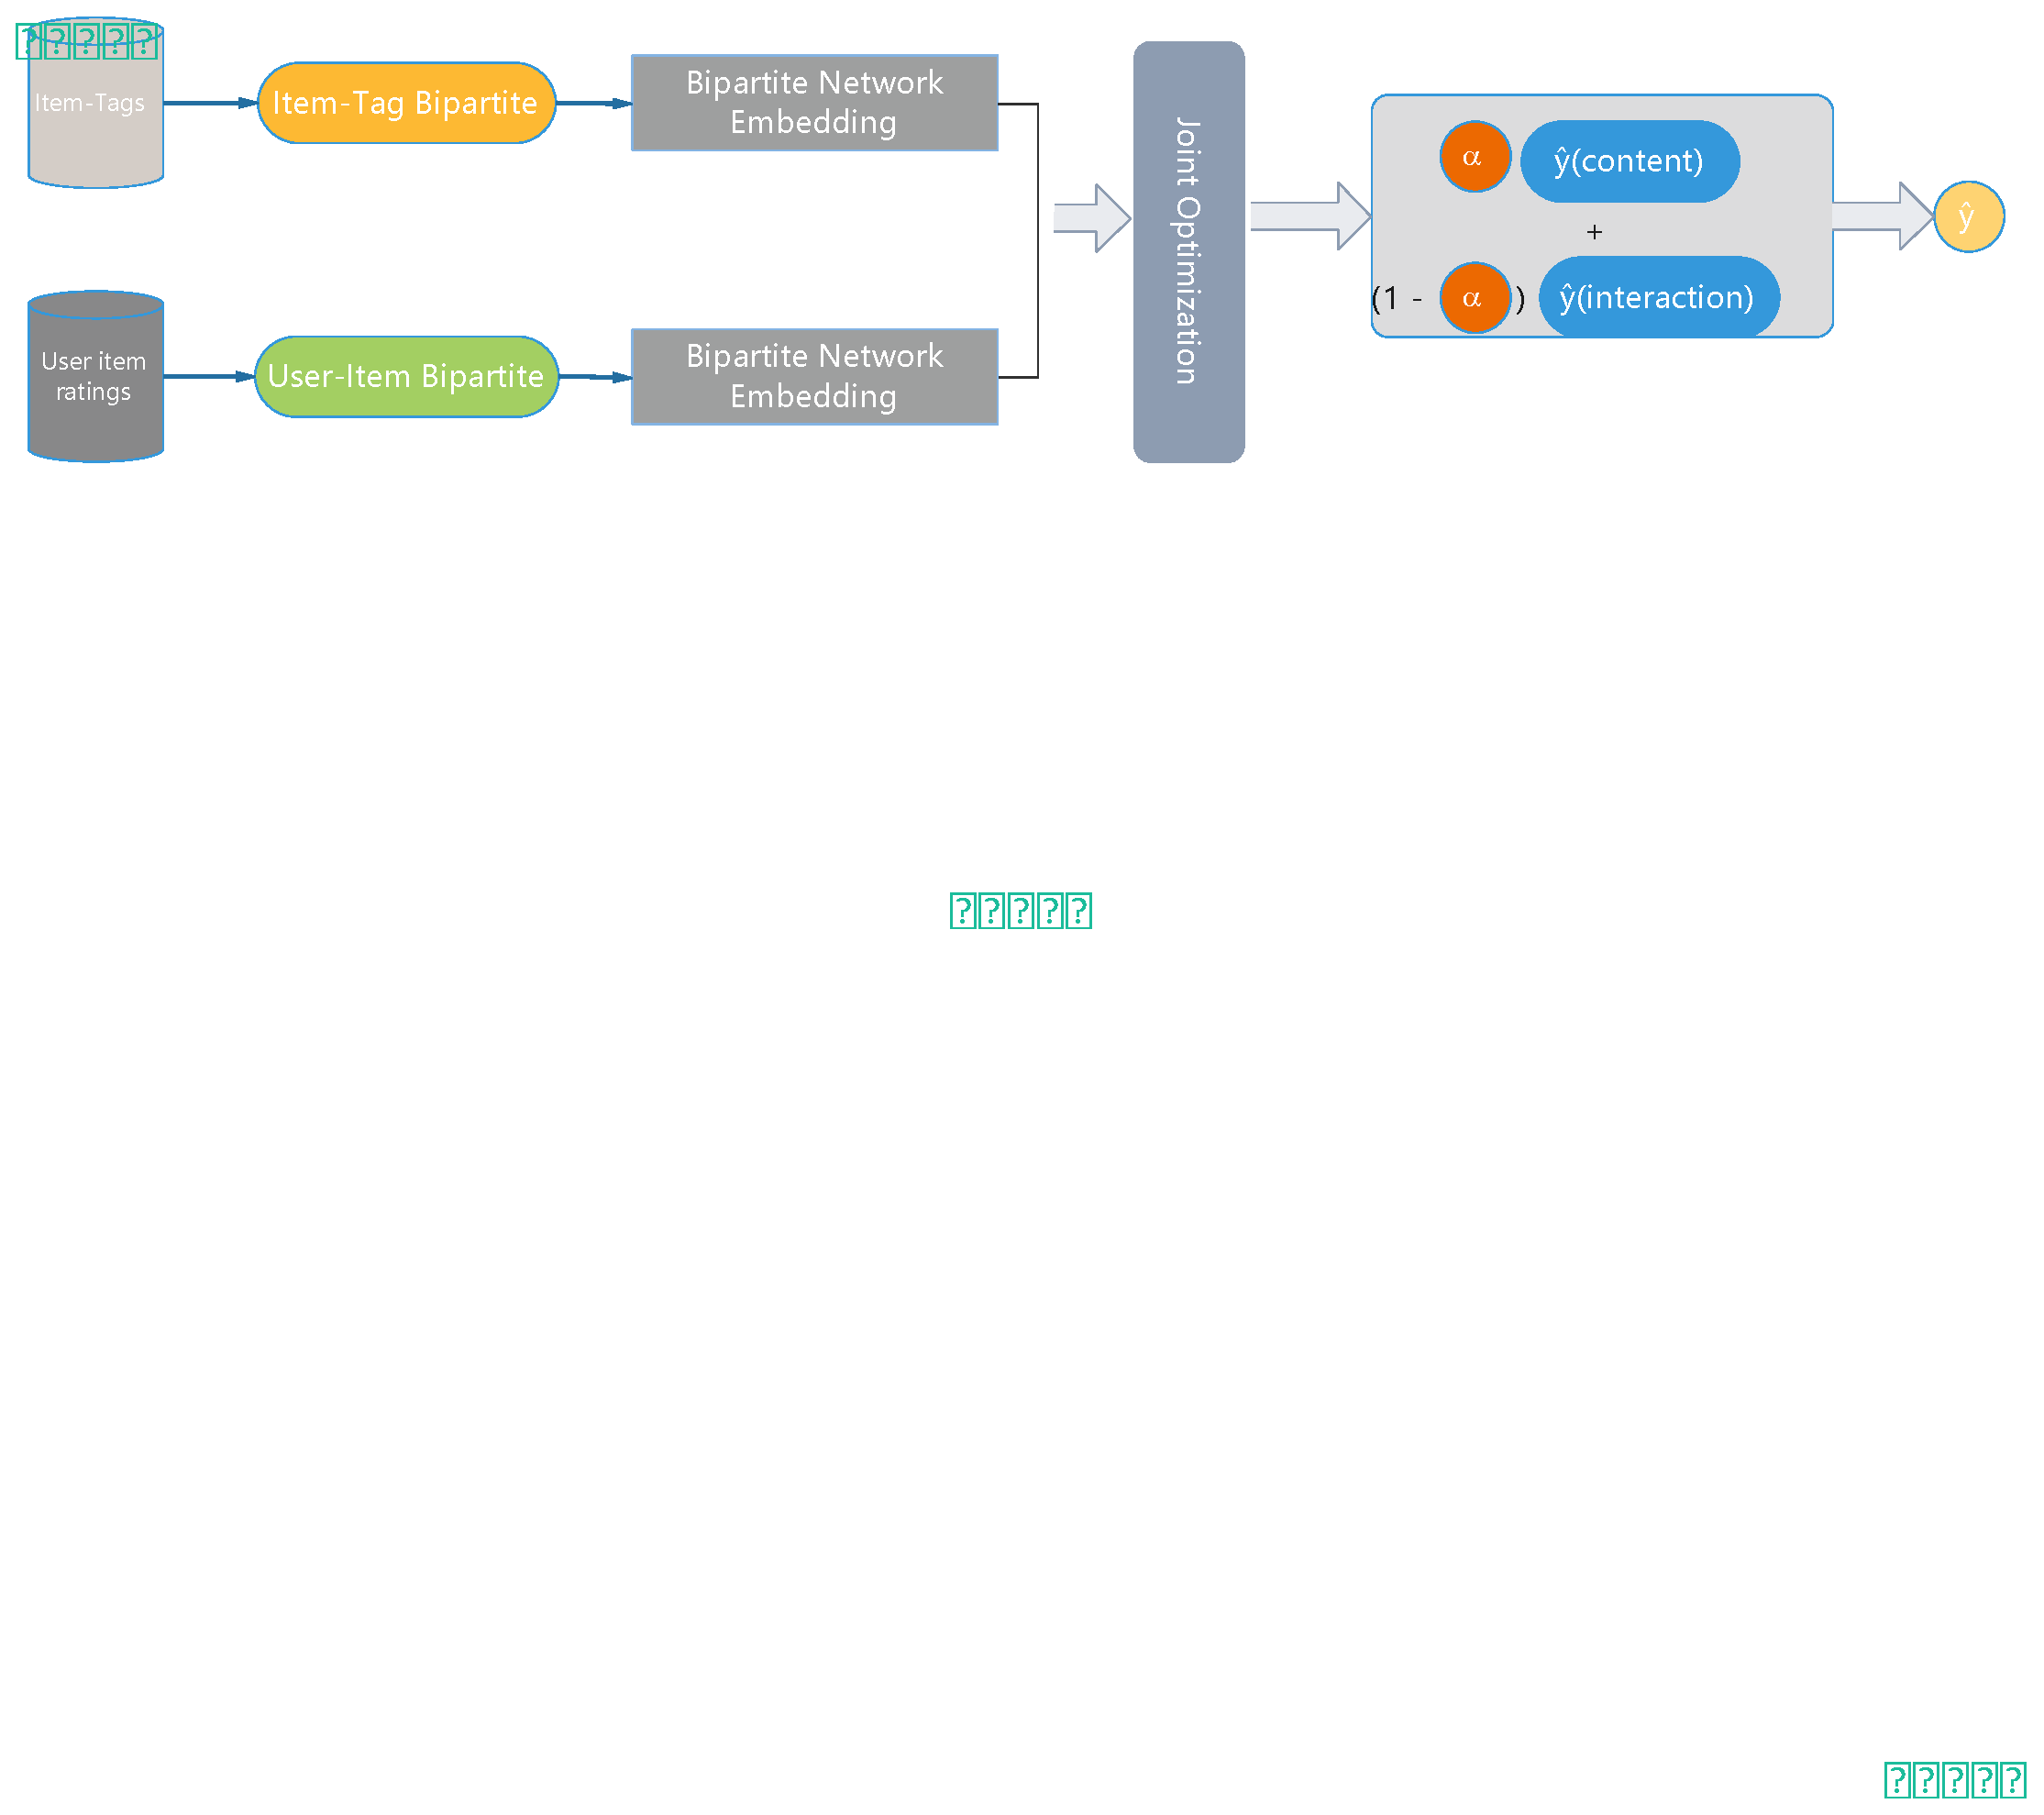
\includegraphics[width=0.6\textwidth]{imgs/framework.eps}

\section{实验}
实验部分,介绍论文的实验

我强烈建议你使用 \lstinline{booktabs} 宏包,这个宏包有三个命令 \lstinline{\toprule}、\lstinline{\midrule} 和 \lstinline{\bottomrule} 能方便你制作三线表。图\ref{fig:scatter} 是一个示例:



\section{结论和未来工作}
结论部分,介绍论文的实验结果

% \nocite{*} 代表显示所有的论文文献 包括文中没有引用的

% 如果想修改参考文献样式(非国标),请把下行取消注释,并换成合适的样式(比如 unsrt,plain 样式)。
\bibliographystyle{unsrt}
\bibliography{wpref}

\end{document}
